Los algoritmos de \textit{clustering basado en grafos}, a diferencia de otros como K-Means o GMM, no aplican un modelo matemático particular para representar el conjunto de datos, o minimizan directamente una función objetivo.
Esto les permite aplicarse en escenarios de mayor complejidad y, en algunos casos, pueden producir clusters de estructura no necesariamente convexa.

La idea detrás de estos algoritmos consiste en construir un grafo no dirigido ponderado $W$, a partir de la matriz de similaridad (o distancias) correspondiente al conjunto de datos.
Para encontrar una partición en $K$ clusters, $A_1,\dots,A_K$, se minimiza la expresión de \textbf{corte} de $W$~\cite{Murphy12}:

\begin{equation}
    \label{eq:graph-cut}
    cut(A_1,\dots,A_K) = \frac{1}{2}\sum_{k=1}^{K}{W(A_k,\bar{A_k})}
\end{equation}

\noindent
donde $V$ son los vértices del grafo (puntos del conjunto de datos), $\bar{A_k}=V\backslash A_k$ es el complemento de $A_k$, y $W(A,B) = \sum_{i\in A, j \in B}{w_{ij}}$.

Frecuentemente ocurre que la solución óptima de~(\ref{eq:graph-cut}) particiona el conjunto separando un único punto del resto.
Para garantizar particiones más razonables, se puede definir el \textbf{corte normalizado}~\cite{Murphy12}:

\begin{equation}
    \label{eq:normalized-cut}
    Ncut(A_1,\dots,A_K) = \frac{1}{2}\sum_{k=1}^{K}{\frac{cut(A_k,\bar{A_k})}{vol(A_k)}}
\end{equation}

\noindent
donde $vol(A_k)=\sum_{i\in A}\sum_{j=1}^{N}{w_{ij}}$.
El problema puede formularse en términos de hallar los vectores de coeficientes binarios $c_i\in{0,1}^N$, donde $c_{ik} = 1$ si el punto $i$ pertenece al cluster $k$, tales que se minimiza $Ncut$~\cite{Murphy12}.
El modo de hallar los vectores $c_i$ distingue los dos algoritmos que más adelante se mencionan: \textbf{Clustering espectral} y \textbf{Affinity propagation}.

\subsection{Matriz de Similaridad}\label{subsec:matrizDeSimilaridad}

La matriz de similitudes entre los puntos del conjunto de datos suele tomarse como la matriz de adyacencia correspondiente a uno de los siguientes grafos denotados por $G$~\cite{Luxburg07,Aggarawal13}:

\begin{enumerate}
    \item \textbf{Grafo de KNN}: Se conectan los puntos $x_i$ y $x_j$ si uno se encuentra entre los $K$ puntos más cercanos al otro.
    La distancia se computa empleando la representación original de los puntos;
    a menudo se utilizan las normas $L_1$ o $L_2$, o la similitud coseno.
    Esto puede hacerse tanto si ambos puntos son $K$-vecinos entre sí, como si uno solo lo es del otro.
    Igualmente el peso de las aristas puede tomarse binario (1 si hay arista, 0 si no) o a partir de la distancia existente entre los puntos.

    \item \textbf{Grafo de $\epsilon$-vecindades}: Dos puntos $x_i$ y $x_j$ se encuentran conectados solo cuando la distancia $|| x_i - x_j ||^2$ es menor que el valor $\epsilon$.

    \item \textbf{Grafo completo}: Todos los puntos con similaridad positiva entre sí son conectados.
    Frecuentemente los pesos de las aristas se definen mediante la función RBF\footnote{\textit{Radial basis function} o \textit{función de base radial} en español.} Gaussiana:
    \[
        W_{ij} = e^{-\sigma \cdot dist(x_i , x_j)^2}
    \]
    donde $dist(x_i , x_j)$ es la distancia euclidiana entre los puntos, y $\sigma$ es un parámetro que determina el decaimiento de la función a medida que los valores se acercan o alejan al 0.
\end{enumerate}

\subsection{Clustering Espectral}\label{subsec:clusteringEspectral}

El clustering espectral se basa en relajar la restricción de que los vectores $c_i$ sean binarios, permitiéndoles tomar valores reales.
Este enfoque convierte el problema en uno de análisis del espectro (vectores propios) de la \textbf{matriz laplaciana} asociada al grafo $W$.

Para cada punto $x_i$, su \textit{grado} puede definirse como la suma de los pesos de las aristas incidentes sobre él:

\begin{equation*}
    d_i = \sum_{j=1}^{n}{W_{ij}}
\end{equation*}

A partir de los grados, puede definirse entonces la \textit{matriz de grados} $D$, como la matriz diagonal que satisface $D_{ii}=d_i$.

Tomando el grafo $W$ como una matriz simétrica, es decir, donde $w_{ij}=w_{ji}\geq 0$, entonces puede definirse la matriz laplaciana asociada a $W$ como:

\begin{equation}
    \label{eq:laplacian-graph}
    L = D - W
\end{equation}

Esta matriz cumple varias propiedades importantes~\cite{Luxburg07}:

\begin{enumerate}
    \item Para todo vector $f\in \mathbb{R}^n$, se cumple que
    \[
        f^T Lf = \frac{1}{2}\sum_{i,j=1}^{n}{W_{ij}(f_i - f_j)^2}
    \]
    \item $L$ es simétrica y semidefinida positiva.
    \item El menor valor propio de $L$ es 0, y el vector propio correspondiente es el vector constante uno, $\mathbbm{1}$.
    \item $L$ tiene $n$ valores propios reales no negativos $0=\lambda_1 \leq \lambda_2 \leq \dots \leq \lambda_n$.
\end{enumerate}

El conjunto de vectores propios, dado por los \textit{vectores indicadores} $\mathbbm{1}_{A_1}, \dots, \mathbbm{1}_{A_K}$, con valores propios 0, se corresponde con las $K$ componentes conexas del grafo.
Si $K=1$, y $f$ es un vector propio con valor propio 0, entonces $0=\sum_{i,j}{w_{ij}(f_i - f_j)^2}$.
Si dos nodos pertenecen a la misma componente conexa entonces $w_{ij}>0$ y por tanto $f_i = f_j$, por lo que se verifica que $f$ es constante para todos los vértices conectados por un camino en el grafo.
En el caso de $K>1$, $L$ estará conformada por una matriz diagonal de bloques $L_k$, en cada uno de los cuales ocurre que existirá un mismo $f$ asociado a sus elementos~\cite{Luxburg07,Murphy12}.

A partir de la observación anterior puede plantearse el algoritmo~\ref{algorithm:UnnormalizedSpectralClustering}.

\begin{algorithm}
    \caption{Clustering Espectral No Normalizado}
    \label{algorithm:UnnormalizedSpectralClustering}
    Construir las matrices $W$ y $D$, de similaridad y grados respectivamente\;
    Computar la matriz laplaciana $L = D-W$\;
    Determinar los primeros $K$ vectores propios $u_k$ de $L$, conformando con ellos la matriz $U = [u_1,\dots,u_k]$ de dimensiones $N\times K$\;
    Aplicar K-Means (u otro algoritmo de clustering) a las filas $y_{i}\in \mathbb{R}^K$ de $U$\;
\end{algorithm}

En el caso ideal en que los clusters se hallen lo suficientemente separados entre sí como para encontrarse reflejados en las $K$ componentes conexas;
entonces, como se mencionó con anterioridad, las filas correspondientes a elementos de una misma componente conexa serán idénticas.
De lo contrario, pueden existir pequeñas perturbaciones que las hagan un poco diferentes, en correspondencia con qué tan distantes se encuentren los respectivos elementos en su espacio original.

\subsubsection{Normalización}

Existen otras dos variantes comunes para la matriz laplaciana que la normalizan~\cite{Aggarawal13}:

\begin{align}
    \label{eq:sym-laplacian}
    L_{sym} & = D^{-\frac{1}{2}}LD^{-\frac{1}{2}} = I - D^{-\frac{1}{2}} W D^{-\frac{1}{2}} \\
    \label{eq:rw-laplacian}
    L_{rw} & = D^{-1}L = I - D^{-1}W
\end{align}

\noindent donde $I$ es la matriz identidad (1 en la diagonal principal y 0 en el resto de las posiciones).

Si se emplea la matriz de~(\ref{eq:rw-laplacian}), el procedimiento es el mismo al mostrado en el algoritmo~\ref{algorithm:UnnormalizedSpectralClustering}, con el paso adicional del cálculo de $L_{rw}$ y empleando esta última en sustitución de $L$.

El uso de $L_{sym}$ es más complicado pues los vectores propios serán de la forma $D^{\frac{1}{2}}\mathbbm{1}_{A_k}$; por ello, antes de aplicar K-Means sobre las filas de la matriz $U$, es necesario normalizarlas creando así la matriz $T$ con $t_{ij} = u_{ij}/\sqrt{\sum_{k}{u_{ik}^2}}$~\cite{Murphy12}.

\subsubsection{Complejidad espacial y temporal}

%TODO Do this!

\subsection{Affinity Propagation}\label{subsec:affinityPropagation}

\textit{Affinity Propagation} es un algoritmo que sigue la idea de que cada punto debe escoger a otro como su \textit{ejemplo} o \textit{centroide};
algunos puntos se elegirán a sí mismos como centroides, y esto automáticamente determinará el número de clusters.

Para este algoritmo se tiene un único vector de coeficientes $c_i \in {1,\dots,N}$ que representan el centroide del punto $i$-ésimo.
El objetivo es maximizar la siguiente función:

\begin{equation}
    \label{eq:affinity-propagation}
    S(c) = \sum_{i=1}^{N}s(i,c_i) + \sum_{k=1}^{K}{\delta_k(c)}
\end{equation}

\noindent
donde $s(i, c_i)$ mide la similaridad entre el punto $i$ y el centroide correspondiente.
El segundo término sirve para penalizar el resultado, siendo $-\infty$ si algún elemento $i$ ha elegido $k$ como centroide ($c_i = k$), pero $k$ no se ha elegido a sí mismo ($c_k \neq k$).
En otras palabras:

\begin{equation}
    \label{affinity-propagation-penalty}
    \delta_k(c) = \begin{cases}
                      -\infty & \text{si $c_k \neq k$ pero $\exists i: c_i = k$} \\
                      0 & \text{eoc.}
    \end{cases}
\end{equation}

Los puntos se envían, con cada uno de los restantes puntos, mensajes que pertenecen a una de dos categorías:
\begin{itemize}
    \item \textit{Responsabilidad} $r(i, k)$: Mide cuánta importancia le asocia el punto $i$ a que $k$ sea su centroide, comparado con otros posibles centroides para $i$.
    \item \textit{Disponibilidad} $a(i, k)$: Indica cuánta importancia le asocia el punto $k$ a ser el centroide de $i$, comparado con otros posibles puntos de los que puede ser centroide.
\end{itemize}

Las responsabilidades y disponibilidades se inicializan en cero para todos los pares de puntos y son actualizadas iterativamente siguiendo las siguientes fórmulas:

\begin{align}
    \label{eq:responsibility}
    r(i,k) &= s(i,k) - \max_{k' \neq k}\left[ a(i, k') + s(i,k') \right] \\
    \label{eq:availability}
    a(i, k) &= \min\left[ 0, r(k,k) + \sum_{i'\notin \{i, k\}}{r(i', k)} \right]
\end{align}

Para evitar oscilaciones numéricas, en cada iteración las responsabilidades y disponibilidades son reajustadas respectivamente mediante las expresiones:

\begin{align}
    \label{eq:responsibility-damping}
    r_{t+1}(i,k) &= \lambda \cdot r_t (i,k) + (1-\lambda)\cdot r_{t+1}(i,k) \\
    \label{eq:availability-damping}
    a_{t+1}(i,k) &= \lambda \cdot a_t (i,k) + (1-\lambda)\cdot a_{t+1}(i,k)
\end{align}

\noindent
donde $t$ indica el número de la iteración correspondiente;
y $\lambda$ ($0.5 \leq \lambda \leq 1$) es una constante conocida como \textit{damping factor}, que pondera la variación de un valor respecto a la iteración anterior.

El número de clusters puede ser controlado ajustando los valores de la diagonal principal de la matriz de similaridad, pues $s(i,i)$ sirve como indicador de la preferencia que se le da a $i$ para que sea centroide.
Frecuentemente el valor $s(i,i)$ se fija como la media de todas las similitudes, para todos los $i$.

\begin{figure}[!h]
    \centering
    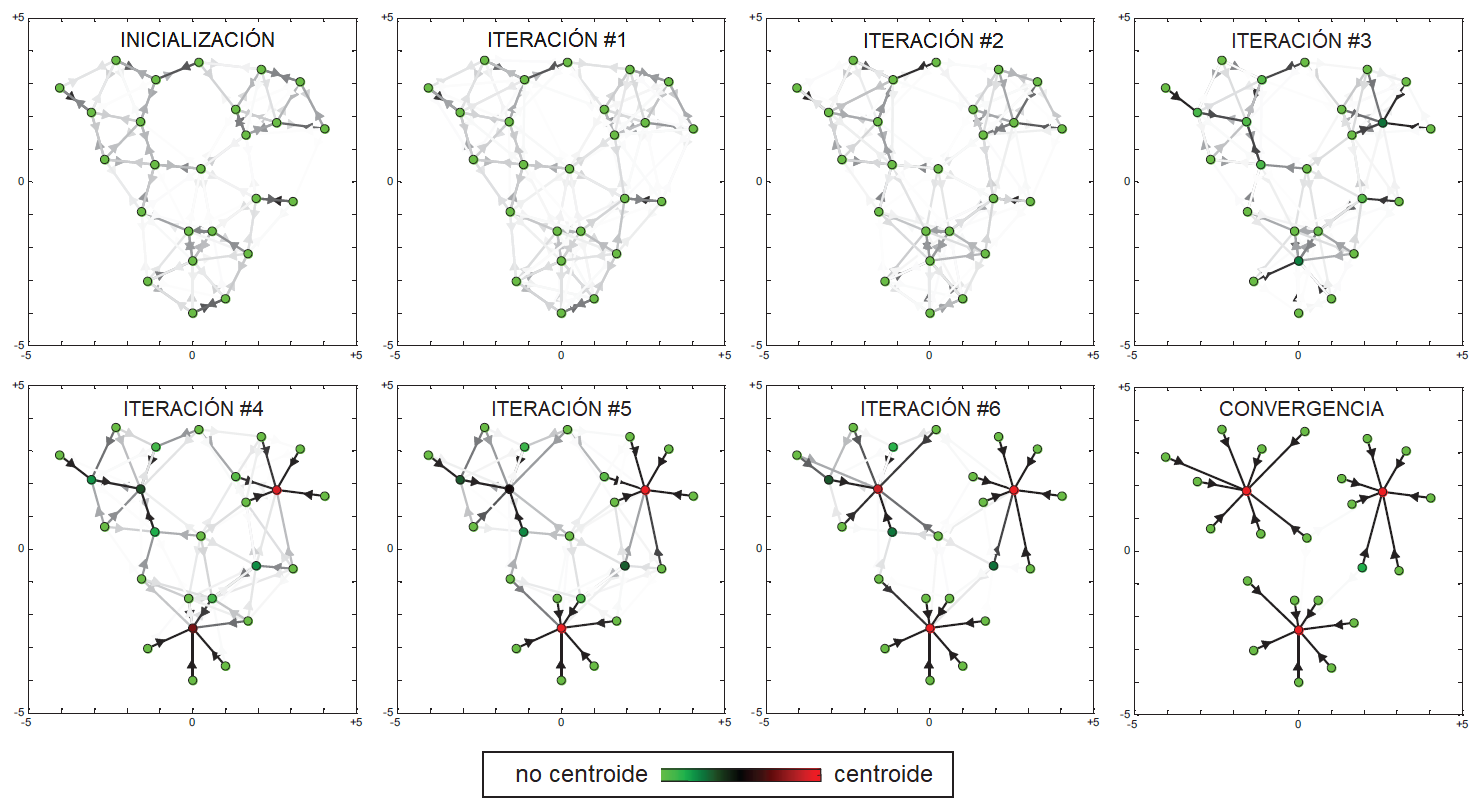
\includegraphics[width=\textwidth]{affinity-propagation.png}
    \caption{Ejemplo de ejecución del algoritmo \textit{Affinity Propagation}. El color de cada punto indica cuán cerca se encuentra de ser centroide. La tonalidad de las flechas refleja la responsabilidad entre sus extremos. (Tomado de~\cite{Murphy12})}
    \label{img:affinity-propagation}
\end{figure}

\subsubsection{Complejidad espacial y temporal}

%TODO Elaborate on this

El algoritmo Affinity Propagation tiene una complejidad temporal $O(N^2 \cdot T)$, con $N$ número de elementos del conjunto de datos y $T$ cantidad de iteraciones hasta converger, para grafos densos.
Para matrices esparcidas (correspondientes a grafos densos), el comportamiento en tiempo del algoritmo es, en cambio, $O(E\cdot T)$, con $E$ número de aristas (valores distintos de cero).

En el caso de la complejidad espacial, la memoria ocupada es $O(N^2)$ y $O(E)$ en dependencia si la matriz es esparcida o no, respectivamente~\cite{Murphy12}.

